\documentclass{beamer}
\beamertemplatenavigationsymbolsempty
\usecolortheme{beaver}
\setbeamertemplate{blocks}[rounded=true, shadow=true]
\setbeamertemplate{footline}[page number]
%
\usepackage[utf8]{inputenc}
\usepackage[english,russian]{babel}
\usepackage{amssymb,amsfonts,amsmath,mathtext}
\usepackage[]{algorithmic}
\usepackage{subfig}
\usepackage[all]{xy} % xy package for diagrams
\usepackage{array}
\usepackage{tikz}
\usepackage{multicol}% many columns in slide
\usepackage{hyperref}% urls
\usepackage{hhline}%tables
% Your figures are here:
\graphicspath{ {fig/} {../fig/} }

%----------------------------------------------------------------------------------------------------------
\title[\hbox to 56mm{Анализ смещения распределений}]{ Анализ смещения распределений при использовании сравнительного подхода в обучении представления данных}
\author[М.\,А. Никитина]{Мария Александровна Никитина}
\institute{Московский физико-технический институт}
\date{\footnotesize
\par\smallskip\emph{Кафедра:} Интеллектуальный анализ данных
\par\smallskip\emph{Научный руководитель:} кандидат ф.-м. наук Р.\,В.~Исаченко
\par\bigskip\small 2024}
%----------------------------------------------------------------------------------------------------------
\begin{document}
%----------------------------------------------------------------------------------------------------------
\begin{frame}
\thispagestyle{empty}
\maketitle
\end{frame}
%-----------------------------------------------------------------------------------------------------
\begin{frame}{Цель исследования}
\begin{block}{Цель}
Оценка распределения данных и устранение смещения распределения
\end{block}
\begin{block}{Задача}
Нахождение оптимальной лосс-функции, устраняющей смещение, и её применение в алгоритме обучения модели.
\end{block}
\begin{block}{Идея}
Выразить распределение положительных элементов через декомпозицию полного распределения:

\[p_x^+ (\textbf{x}') = \frac{p(\textbf{x}') - \tau^- p^-_x(\textbf{x}')}{\tau^+},\]

где $\tau^+$, $\tau^-$ -- вероятности нахождения положительных и отрицательных элементов соответственно.
\end{block}
\end{frame}
%-----------------------------------------------------------------------------------------------------
\begin{frame}{Contrastive learning}
\textit{Contrastive learning} – подход при котором обучение происходит не только по принципу близости, но и по принципу различия.

\bigskip

Положим вектор $\textbf{x}$ некоторого объекта в качестве основного. Тогда вектор схожего объекта назовём $\textbf{x}^+$ -- позитивный элемент. Он должен быть как можно ближе к $\textbf{x}$. А вектор отличного объекта $\textbf{x}^-$ -- как можно дальше, как негативный элемент.
\begin{figure}
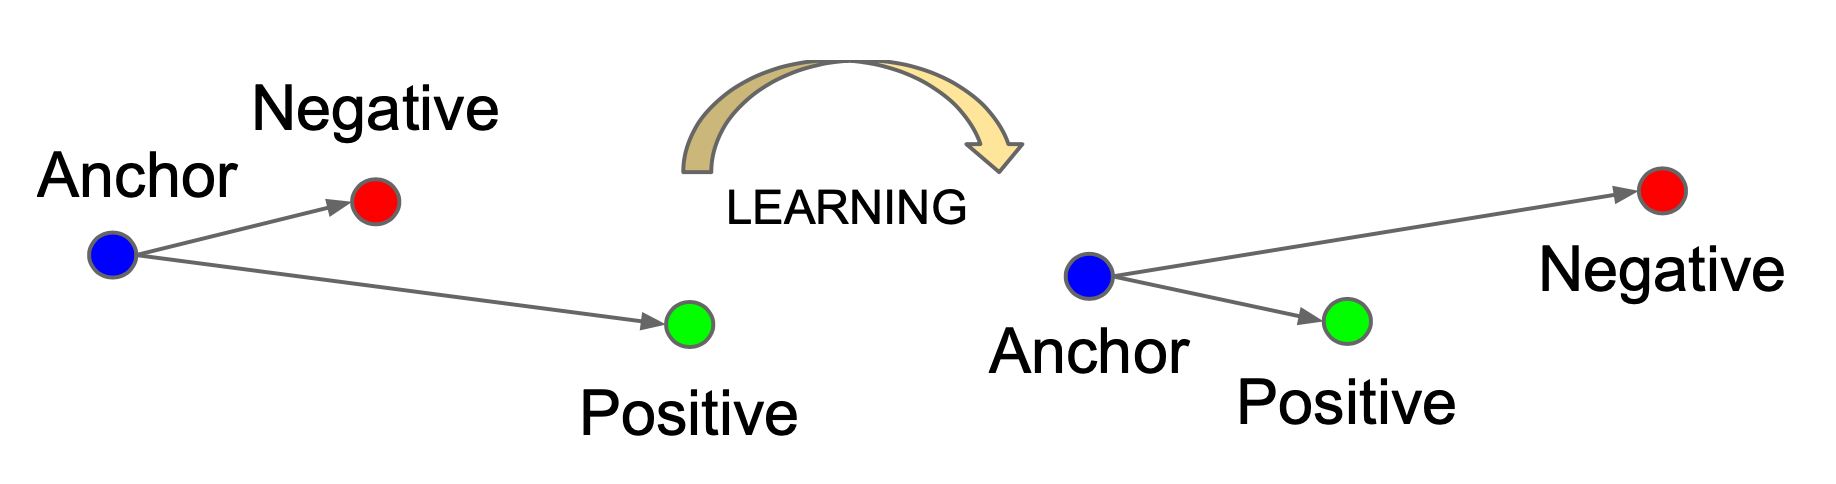
\includegraphics[width=7cm]{Presentation/triplet-loss.png}
\caption{Принцип contrastive learning. Взято из [Schroff et al. 2015].}
\end{figure}
\end{frame}


%----------------------------------------------------------------------------------------------------------
\begin{frame}{Список литературы}
\begin{thebibliography}{99} 
    \footnotesize
    
    \bibitem[Chuang, 2020]{p1}
        Ching-Yao Chuang, Joshua Robinson, Lin Yen-Chen, Antonio Torralba, Stefanie Jegelkah (2020)
        \newblock Debiased Contrastive Learning

        \bibitem[khosla2021supervised, 2020]{p2}
        Prannay Khosla, Piotr Teterwak, Chen Wang, Aaron Sarna, Yonglong Tian, Phillip Isola, Aaron Maschinot, Ce Liu, Dilip Krishnan (2021)
        \newblock Supervised Contrastive Learning

       \bibitem[Chen2020SimCLR, 2020]{p3}
        CTing Chen, Simon Kornblith, Mohammad Norouzi, Geoffrey Hinton (2020)
        \newblock A Simple Framework for Contrastive Learning of Visual Representations

    \bibitem[VQA, 2017]{p4}
        Stanislaw Antol and Aishwarya Agrawal and Jiasen Lu and Margaret Mitchell and Dhruv Batra and C. Lawrence Zitnick and Devi Parikh
        \newblock {VQA}: {V}isual {Q}uestion {A}nswering

    \bibitem[schroff2015facenet, 2015]{p5}
        Florian Schroff, Dmitry Kalenichenko, James Philbin (2015)
        \newblock FaceNet: A Unified Embedding for Face Recognition and Clustering

\end{thebibliography}
\end{frame}
%----------------------------------------------------------------------------------------------------------
\begin{frame}{Ложноположительные и ложноотрицательные элементы}
Классический лосс, не учитывающий смещения:
\[\mathcal{L}_{N-pair}(f) = - \log \frac{\exp(f(\textbf{x})^T f(\textbf{x}_i^+))}{\exp(f(\textbf{x})^T f(\textbf{x}_i^+)) + \sum _{i=1}^{N} \exp(f(\textbf{x})^Tf(\textbf{x}_i^-))}\]

Решение для устранения смещения ложноотрицательных элементов [Chuang et al., 2020]:

\begin{equation*} \small
L_{\text{Neg}}^{N, M}(f) = \mathbb{E}_{\substack{\textbf{x} \sim p; \textbf{x}_+ \sim p_x^+,\\ \{\textbf{u}_i\}_{i=1}^N \sim p^N \\ \{\textbf{v}_j\}_{j=1}^M \sim {p_x^+}^M}}  \bigg[ -\log \frac{e^{f(\textbf{x})^T f(\textbf{x}^+)} }{e^{f(\textbf{x})^T f(\textbf{x}^+)} + N g\big(\textbf{x}, \{\textbf{u}_i\}_{i=1}^N, \{\textbf{v}_j\}_{j=1}^M\big)} \bigg]
\end{equation*}

\begin{figure}
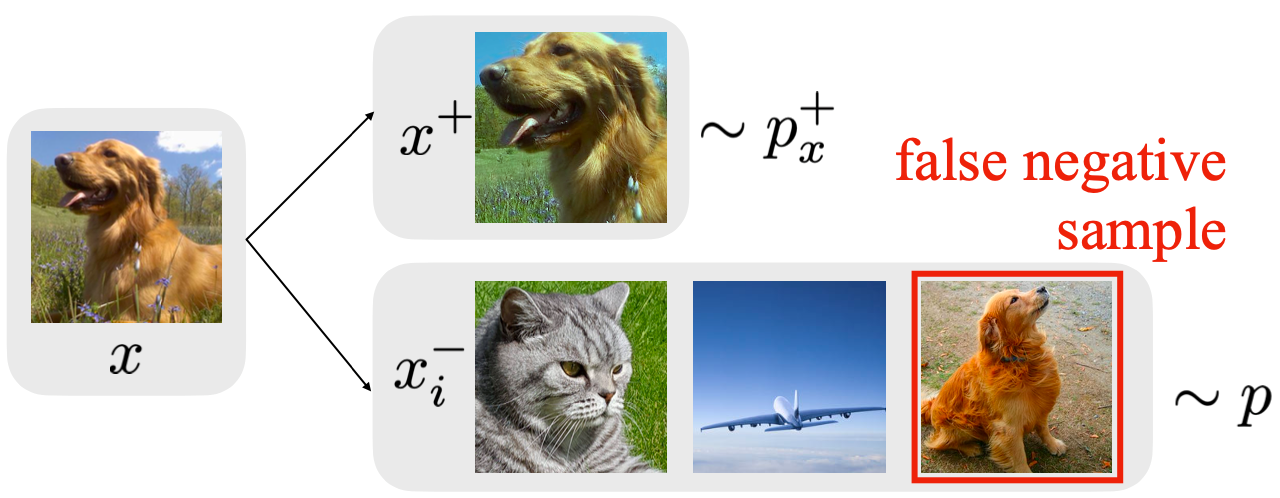
\includegraphics[width=6cm]{Presentation/contrastive-sampling-bias.png}
\caption{Взято из [Chuang et al., 2020].}
\end{figure}
\end{frame}
%----------------------------------------------------------------------------------------------------------
\begin{frame}{DebiasedPos}
\scriptsize
В отличие от $L_{\text{Neg}}^{N, M}(f)$ здесь устраняется смещение ложноположительных элементов.
\begin{equation*}
\tilde{L}_{\text{Pos}}^N (f) = \mathbb{E}_{\substack{\textbf{x} \sim p \\ \textbf{x}^- \sim p_x^-}} \bigg[ - \log \frac{\color{violet} \mathbb{E}_{\textbf{x}' \sim p} f(\textbf{x}, \textbf{x}') \color{black} - \tau^- \color{blue} \mathbb{E}_{\textbf{x}^- \sim p_x^-} f(\textbf{x}, \textbf{x}_i^-)}{\color{violet} \mathbb{E}_{\textbf{x}' \sim p} f(\textbf{x}, \textbf{x}') \color{black} + \big(N \tau^+ - \tau^-\big) \color{blue} \mathbb{E}_{\textbf{x}^- \sim p_x^-} f(\textbf{x}, \textbf{x}_i^-)}\bigg]
\end{equation*}

Финальная оценка:
\begin{equation*}
L_{\text{Pos}}^N (f) = \mathbb{E}_{\substack{\textbf{x} \sim p \\ \{\textbf{u}_i\}_{i=1}^N \sim {p_x^-}^N \\ \textbf{v} \sim p_x^+}} \bigg[-\log \frac{\color{violet}P_{\text{emp}} \color{black} - \tau^- \color{blue} P_{\text{emp}}^-} {\color{violet}P_{\text{emp}} \color{black} + \big(N \tau^+ - \tau^-\big) \color{blue} P_{\text{emp}}^- }\bigg].
\end{equation*}

$P_{\text{emp}}$, $P_{\text{emp}}^-$ --эмпирические оценки матожиданий.
\end{frame}

%----------------------------------------------------------------------------------------------------------
\begin{frame}{Оценки}
\begin{lemma}
% \normalfont 
При $N \to \infty$:
$$\mathcal{L}_{\text{N-pair}}^N(f) \to \tilde{L}_{\text{Pos}}^N (f)$$
\end{lemma}

\begin{theorem}
$\mathcal{L}_{\text{Pos}}^N$ максимизирует нижнюю границу взаимной информации.
$$I(x, c) = \sum\limits_{x \in X, c \in C}p(x, c)\log \frac{p(x|c)}{p(x)} \geq$$
$$\geq \mathbb{E}_{x \sim p}\log\left((N + 2)\frac{p(x|c)}{p(x)}\right) - \mathcal{L}_{\text{Pos}}^N$$
\end{theorem}
\end{frame}
%----------------------------------------------------------------------------------------------------------
\begin{frame}{SimCLR}
\framesubtitle{CTing Chen et. al., 2020} % Optional subtitle

\begin{figure}
    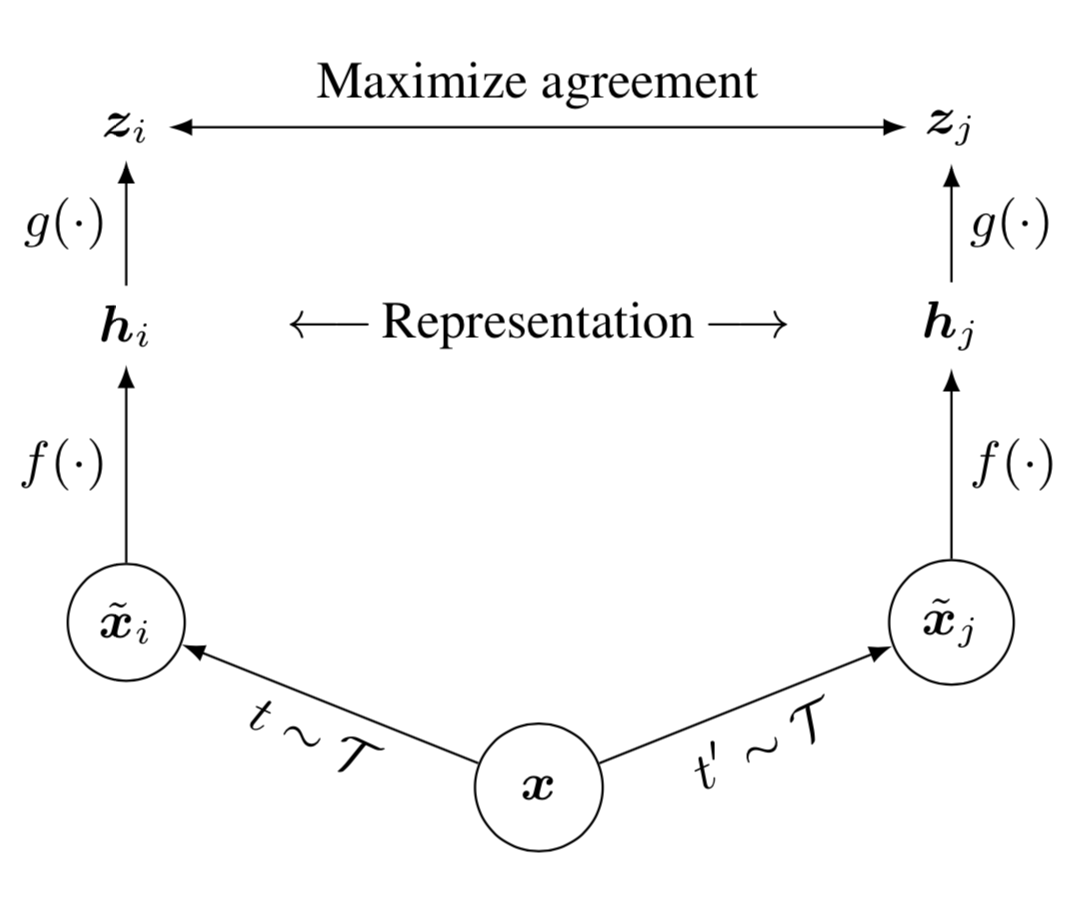
\includegraphics[width=0.5\linewidth]{Presentation/SimCLR.png}
\end{figure}

\scriptsize
\begin{itemize}
    \item $\mathcal{T} -$ семейство аугментаций
    \item Семплируются 2 аугментации $t, t' \sim \mathcal{T}$, применяются к каждому объекту.
    \item Обучаем сеть-энкодер $f(\cdot)$ и MLP сеть-проекцию $g(\cdot)$, максимизируя соответствие представлений.
\end{itemize}
\end{frame}
%----------------------------------------------------------------------------------------------------------
\begin{frame}{Вычислительный эксперимент}
\begin{block}{Цель}
Сравнить работу $L_{\text{Neg}}^N(f)$, $L_{\text{Pos}}^N(f)$ и $L_{N-pair}(f)$ на модели SimCLR.
\end{block}

\begin{block}{Первичный результат}
\begin{figure}
   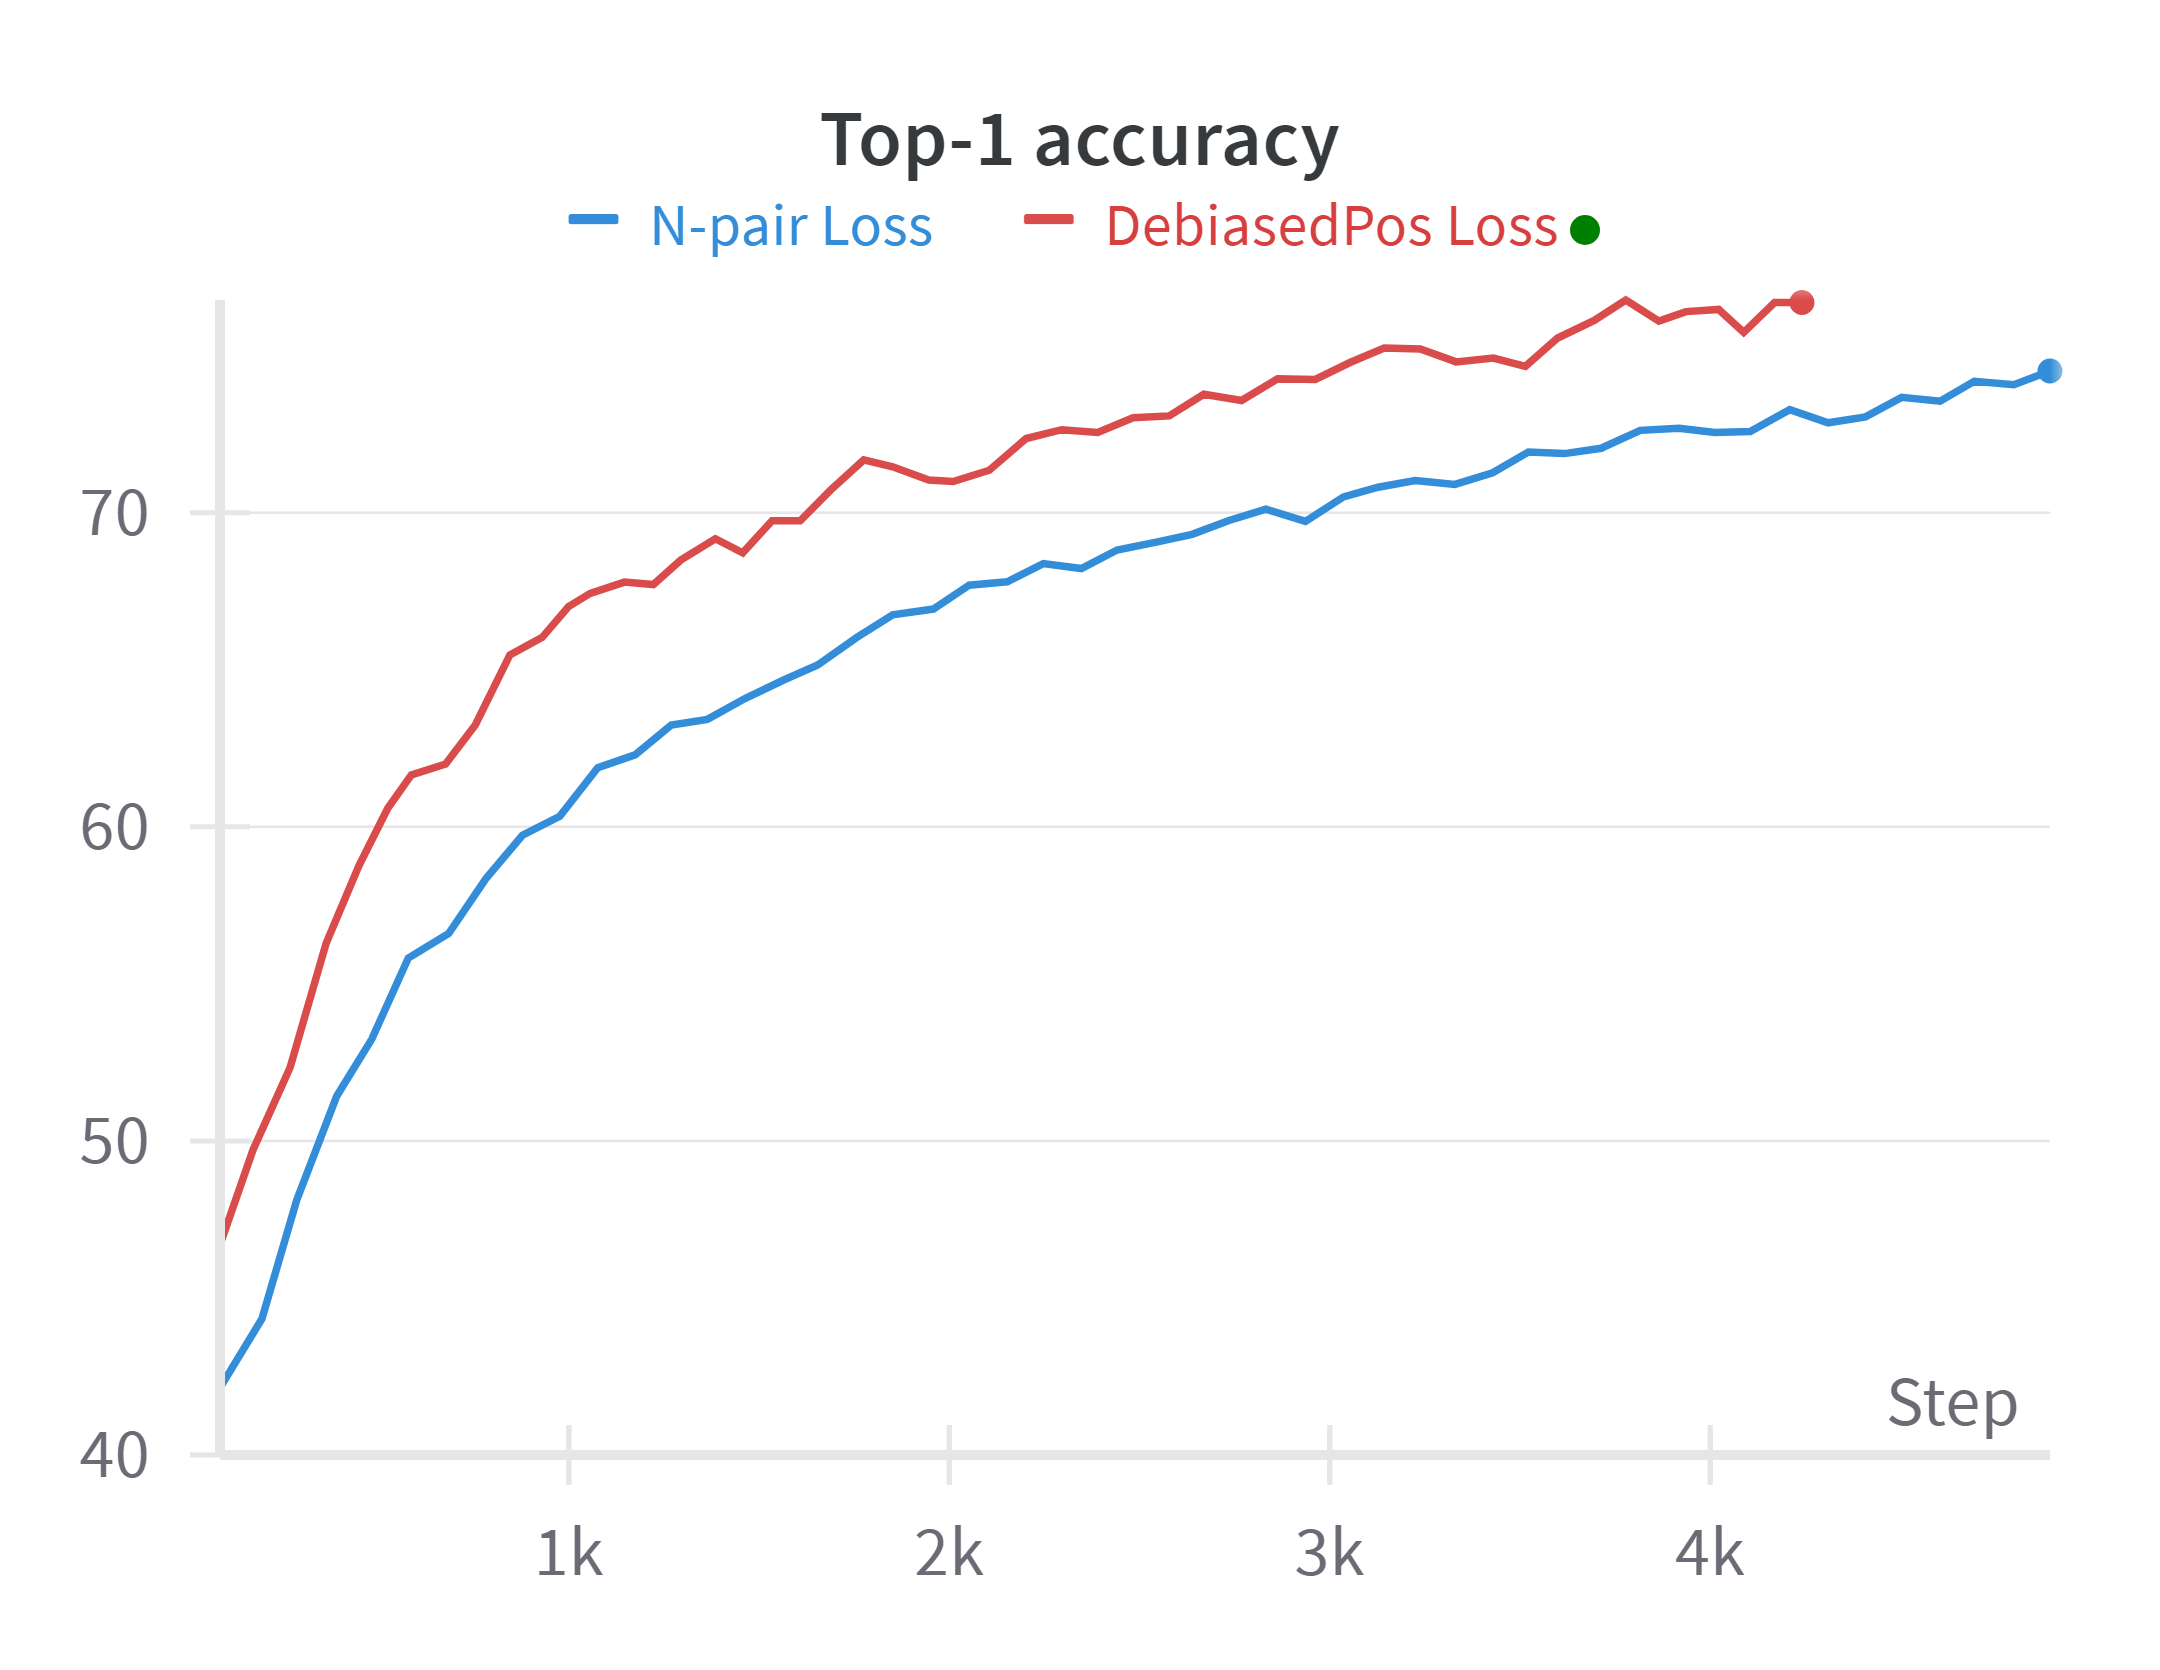
\includegraphics[width=0.475\textwidth]{Presentation/W&B Chart 14.12.2023, 18_23_46 (1).png}
   \hfill
   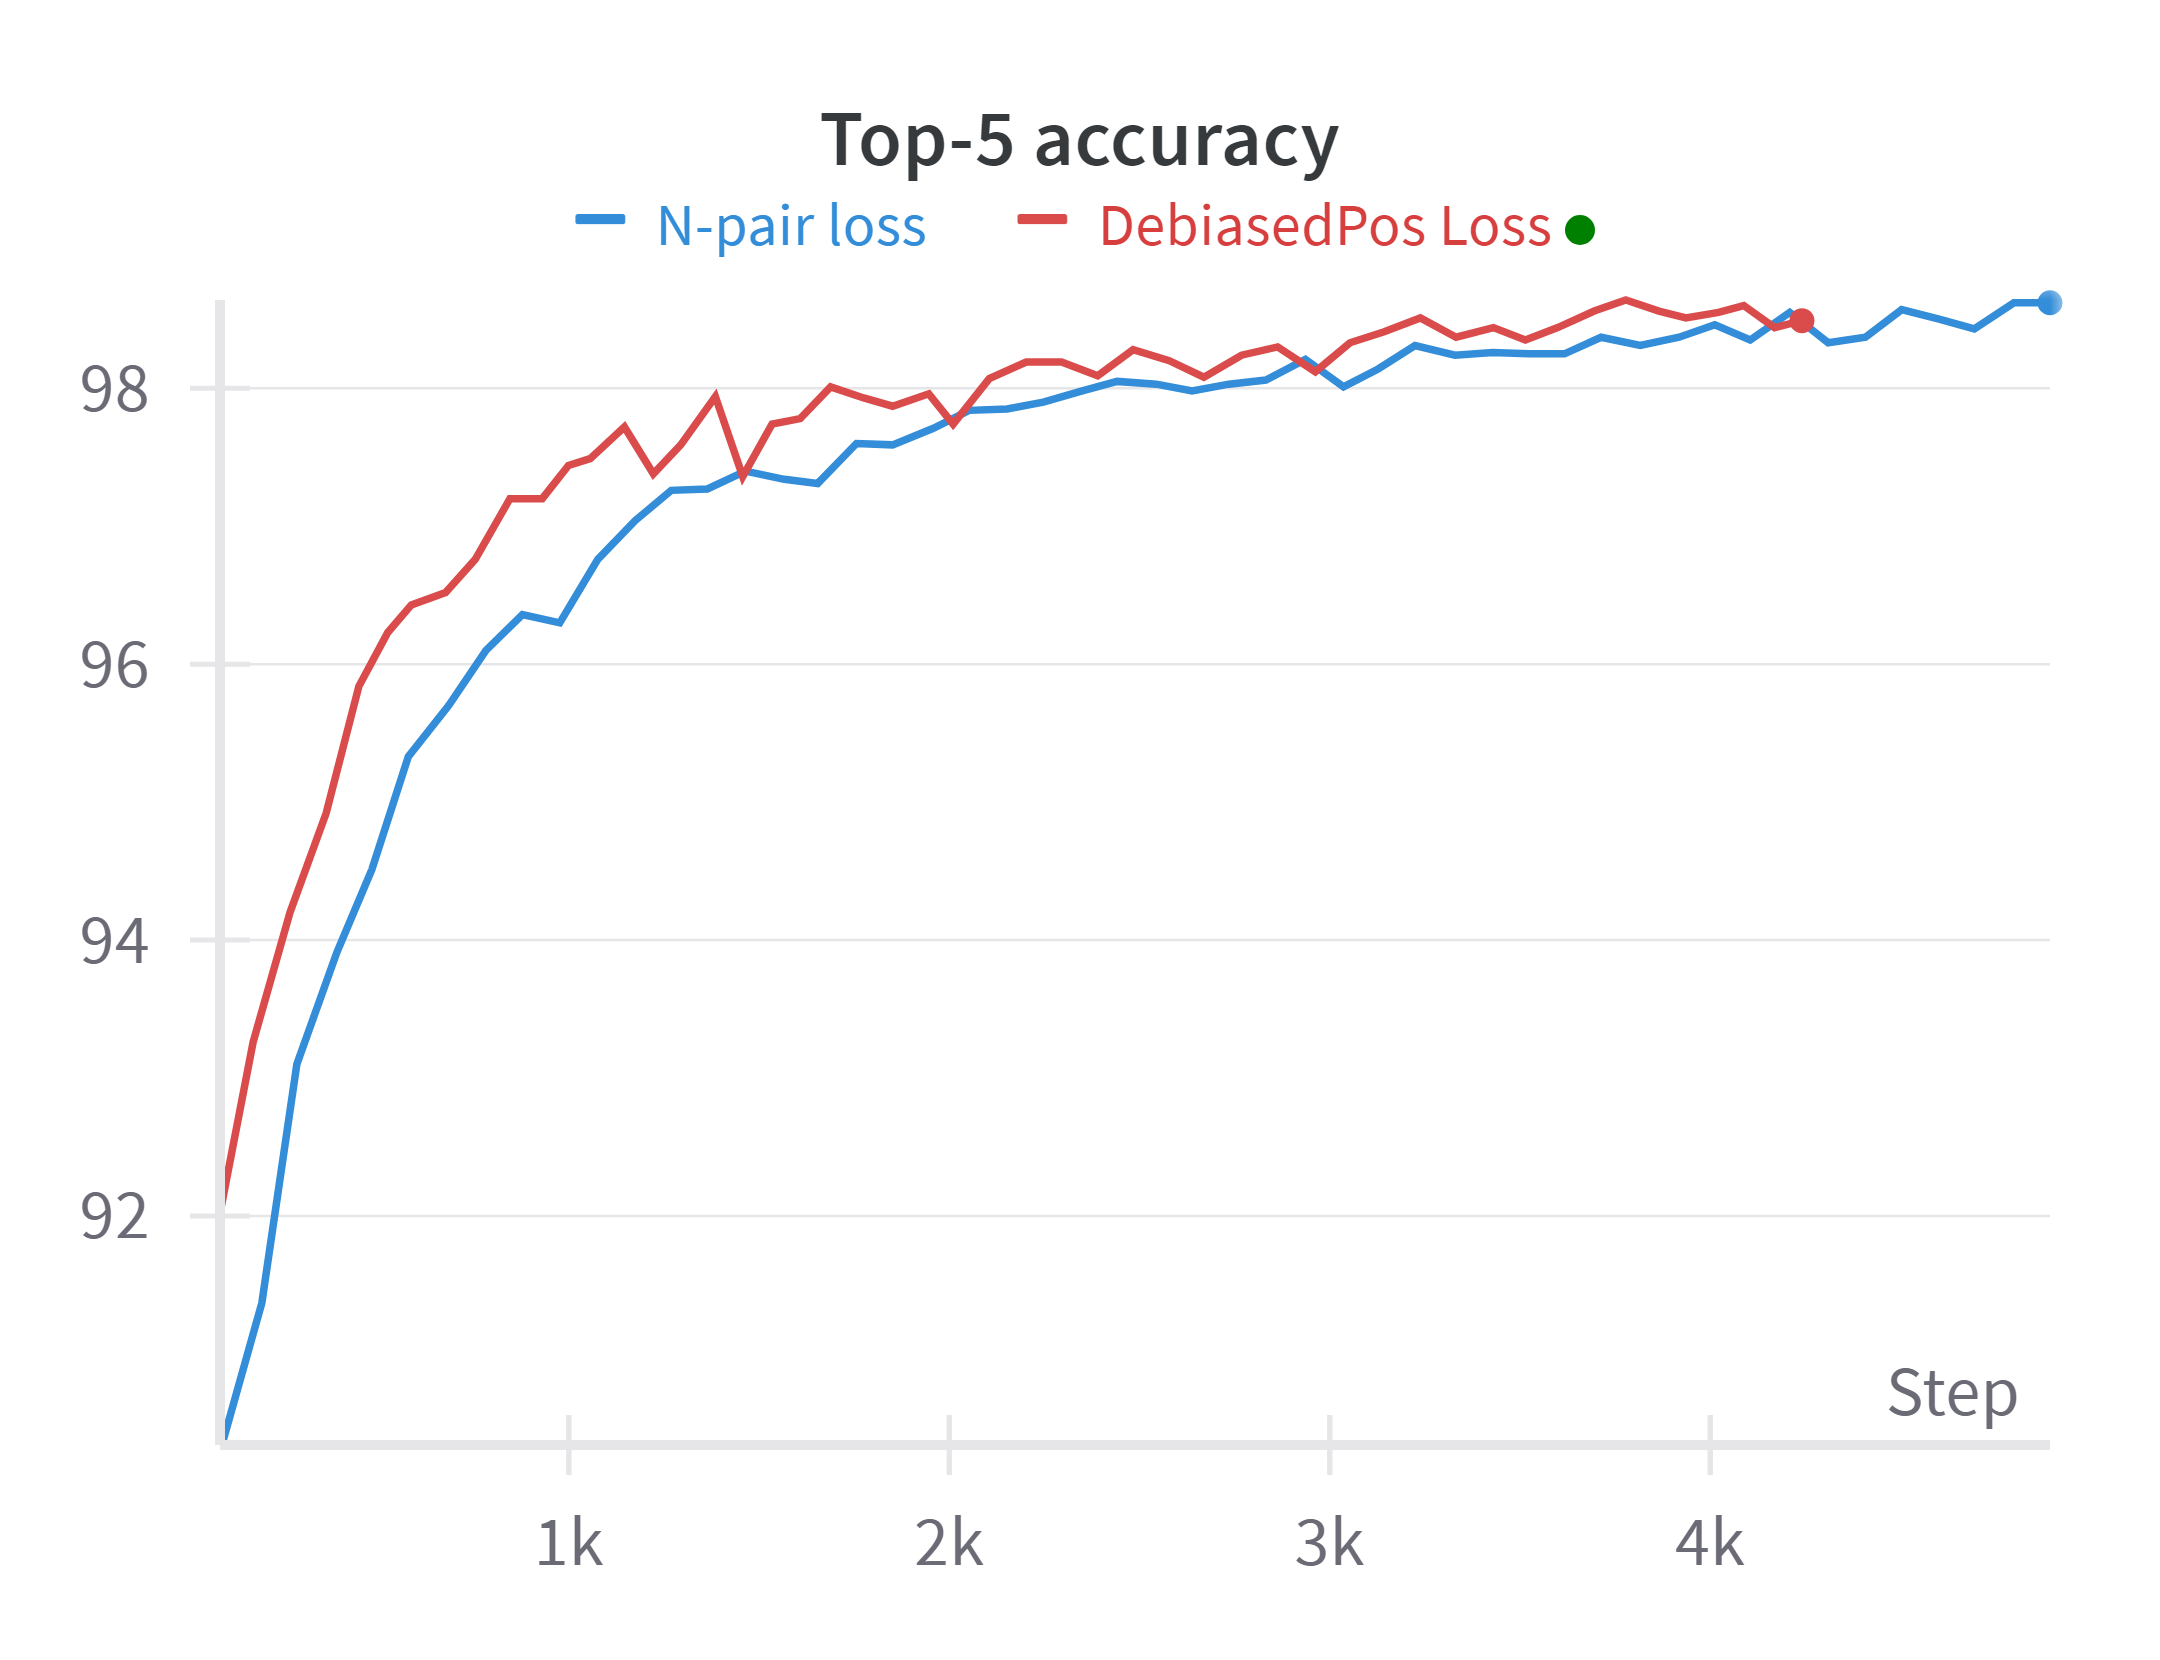
\includegraphics[width=0.475\textwidth]{Presentation/W&B Chart 14.12.2023, 18_29_05.png}
\end{figure}
\end{block}

\end{frame}
%----------------------------------------------------------------------------------------------------------
\begin{frame}{VQA} 
\begin{block}{Цель}
Сравнить работу $L_{\text{Pos}}^N(f)$ и $L_{N-pair}(f)$ на большой задаче Visual Question Answering [Stanislaw Antol et. al.]
\end{block}
\end{frame}
%----------------------------------------------------------------------------------------------------------
\end{document} 